\documentclass[12pt, letterpaper]{article}
\usepackage{siunitx}
\usepackage{setspace}
\usepackage{gensymb}
\usepackage{xcolor}
\usepackage{caption}
\doublespacing
\singlespacing
\usepackage[none]{hyphenat}
\usepackage{amssymb}
\usepackage{relsize}
\usepackage[cmex10]{amsmath}
\usepackage{mathtools}
\usepackage{amsthm}
\interdisplaylinepenalty=2500
\usepackage{txfonts}
\usepackage{wasysym}
\usepackage{mathrsfs}
\usepackage{stfloats}
\usepackage{float}
\usepackage{cite}
\usepackage{cases}
\usepackage{subfig}
\usepackage{longtable}
\usepackage{multirow}
\usepackage{enumitem}
\usepackage{mathtools}
\usepackage{listings}
\usepackage[latin1]{inputenc}
\usepackage{textcomp}
\usepackage{titling}
\usepackage{hyperref}
\usepackage{tikz}
\usepackage{graphicx}
\lstset{
  frame=single,
  breaklines=true
}
\usepackage{tfrupee}
\usepackage{wrapfig}
\graphicspath{{figs/}}

\providecommand{\mydet}[1]{\ensuremath{\begin{vmatrix}#1\end{v\matrix}}}
\providecommand{\myvec}[1]{\ensuremath{\begin{bmatrix}#1\end{b\matrix}}}
\providecommand{\cbrak}[1]{\ensuremath{\left\{#1\right\}}}
\providecommand{\brak}[1]{\ensuremath{\left(#1\right)}}

\begin{document}
\begin{enumerate}
    \section*{Trigonometry}
    \item If a tower $30$ meters high casts a shadow $10\sqrt{3}$ meters long on the ground, what is the angle of elevation of the sun?

    \section*{Probability}
    \item The probability of selecting a rotten apple randomly from a heap of 900 apples is 0.18. What is the number of rotten apples in the heap?

    \section*{Progressions}
    \item What is the common difference of an A.P. in which $a_{21} + a_{7} = 84$?
    \item Which term of the A.P. $8, 14, 20, 26, \ldots$ will be 72 more than its 41st term?

    \section*{Geometry}
    \item If the angle between two tangents drawn from an external point $P$ to a circle of radius $a$ and center $O$ is $60\degree$, then find the length of $OP$.
    \item Prove that the tangents drawn at the endpoints of a chord of a circle make equal angles with the chord.
    \item A circle touches all the four sides of a quadrilateral $ABCD$. Prove that $AB + CD = BC + DA$.
    \item The dimensions of a solid iron cuboid are $4.4 \times 2.6 \times 10$. It is melted and recast into a hollow cylindrical pipe of $30\,\mathrm{cm}$ inner radius and thickness $5\,\mathrm{cm}$. Find the length of the pipe.
    \item In the given figure, two concentric circles with center $O$ have radii $21\,\mathrm{cm}$ and $42\,\mathrm{cm}$. If $\angle AOB = 60\degree$, find the area of the shaded region.

    \begin{figure}[H]
        \centering
        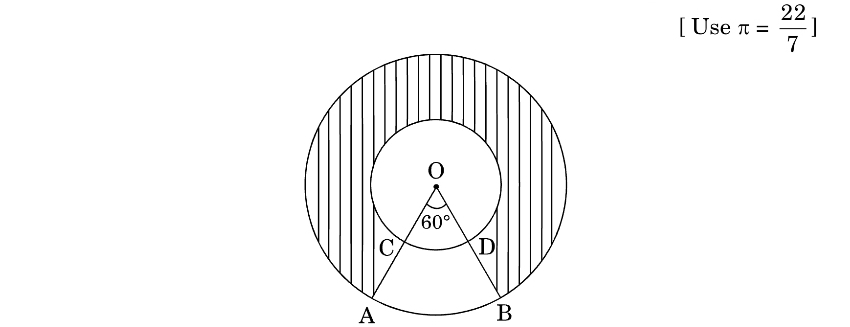
\includegraphics[width=\columnwidth]{final1.jpg}
	    \caption{final1}
    \end{figure}

    \item Water in a canal, $5.4$ wide and $1.8$ deep, is flowing with a speed of $25\mathrm{km/hour}$. How much area can it irrigate in $40$ minutes, if $10\,\mathrm{cm}$ of standing water is required for irrigation?
    \item In what ratio does the point $ \left(\frac{24}{11}, y \right) $ divide the line segment joining the points $P(2, 2)$ and $Q(3, 7)$? Also, find the value of $y$.
    \item On a straight line passing through the foot of a tower, two points $C$ and $D$ are at distances of $4\,\mathrm{m}$ and $16\mathrm{m}$ from the foot respectively. If the angles of elevation from $C$ and $D$ of the top of the tower are complementary, then find the height of the tower.

    \section*{Coordinate Geometry}
    \item A line intersects the y-axis and x-axis at the points $P$ and $Q$ respectively. If $(2,5)$ is the mid-point of $PQ$, then find the coordinates of $P$ and $Q$.
    \item If the distances of $P(x, y)$ from $A(5, 1)$ and $B(-1, 5)$ are equal, then prove that $3x = 2y$.

    \section*{Polynomial}
    \item Find the value of $p$, for which one root of the quadratic equation $p \cdot x^2 - 14x + 8 = 0$ is 6 times the other.
\end{enumerate}
\end{document}

